\subsection{Fundamental Particles}

The fundamental particles are categorised by several intrinsic properties which can be seen in table \ref{fig: particle table}. By their intrinsic spin they are classified as particles with half-integer spin (fermions) and integer spin (bosons), these are outlined in the following sections.

\subsection*{Fermions}
Fermions are further sub-divided into two groups - quarks and leptons - depending on the types of interactions they experience. Quarks have the property of colour which makes them sensitive to the strong interaction whilst leptons do not. 

Both quarks and leptons are further sub-divided into three generations; the higher generations correspond to particles with higher mass states, these particles rapidly decay to the lower stable generations by the weak force. 

Each fermion generation consists of a particle doublet, for example the first generation of quarks is composed of up and down type quarks. Particles in fermions doublets couple strongly to one another such that interactions between the two particle types are relatively strong in comparison to coupling between particles in different generations. This can be seen in the CKM matrix (a matrix which describing coupling between different quark types measured through experiment) where the coupling between the �up� and �down� quarks is  approximately four times greater than between �up� and �strange� type quarks. 

The lepton generations are made up of a charged lepton and neutrino doublet. There is no coupling between lepton generations (in contrast to quarks) in the standard model; higher generation lepton states such as the tau lepton may decay via tree processes such as a decay to its corresponding neutrino along with a $\mathrm{W}^\pm$ boson (see subsection below).

The three generations together with the corresponding doublets gives a total of 6 quark flavours and 6 lepton flavours.

\subsection*{Bosons}
The Standard Model describes two types of bosons, gauge bosons and the Higg's boson. 

A gauge boson is a force carrying particle - also referred to as a force mediator - associated to a particular type of interaction e.g. gluons are associated with the strong interaction and photons are associated to the electromagnetic interaction. The term ``gauge'' comes from the property of the equations of motion related to a given interaction; these are invariant under ``gauge'' transformations which are discussed in section \ref{section: gauge theories}.

The Higg�s boson plays a unique role in the Standard Model. Its existence supports the validity of the Higg�s mechanism; a mechanism which explains why some particles are massive while others are not, in addition to why interaction strengths vary for different interaction types. On the 4th July 2012 the discovery of particle with a mass between 125 and 127 GeV was announced; on the 14th March 2013 the properties of the newly discovered particle were found to be consistent with the Higg�s Boson predicted by the standard model.

\begin{figure}[h]
	\centering
	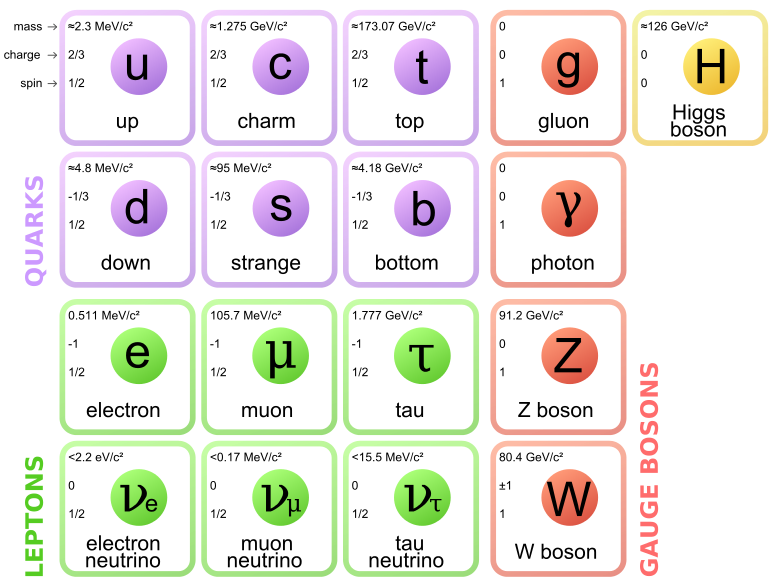
\includegraphics[width=0.75\textwidth]{./Chapters/theory/standard_model/images/particle_table.png}
	\caption{Table of particles in the Standard Model \cite{particle_table}}
	\label{fig: particle table}
\end{figure}